\documentclass[12pt]{article}
\usepackage[margin=2.5cm]{geometry}
\usepackage{enumerate}
\usepackage{amsfonts}
\usepackage{amsmath}
\usepackage{fancyhdr}
\usepackage{amsmath}
\usepackage{amssymb}
\usepackage{amsthm}
\usepackage{mdframed}
\usepackage{graphicx}
\usepackage{subcaption}
\usepackage{adjustbox}
\usepackage{listings}
\usepackage{xcolor}
\usepackage{booktabs}
\usepackage[utf]{kotex}
\usepackage{hyperref}

\definecolor{codegreen}{rgb}{0,0.6,0}
\definecolor{codegray}{rgb}{0.5,0.5,0.5}
\definecolor{codepurple}{rgb}{0.58,0,0.82}
\definecolor{backcolour}{rgb}{0.95,0.95,0.92}

\lstdefinestyle{mystyle}{
    backgroundcolor=\color{backcolour},
    commentstyle=\color{codegreen},
    keywordstyle=\color{magenta},
    numberstyle=\tiny\color{codegray},
    stringstyle=\color{codepurple},
    basicstyle=\ttfamily\footnotesize,
    breakatwhitespace=false,
    breaklines=true,
    captionpos=b,
    keepspaces=true,
    numbers=left,
    numbersep=5pt,
    showspaces=false,
    showstringspaces=false,
    showtabs=false,
    tabsize=1
}

\lstset{style=mystyle}

\pagestyle{fancy}
\renewcommand{\headrulewidth}{0.4pt}
\lhead{CSC 209}
\rhead{Review 9 Solution}

\begin{document}
\title{CSC 209 Review 9 Solution}
\maketitle

\bigskip

\begin{enumerate}[1.]
    \item

    \begin{enumerate}[a)]
        \item 0
        \item
    \end{enumerate}

    \bigskip

    \underline{\textbf{Notes}}

    \begin{itemize}
        \item \texttt{a)} is 0 because  (\texttt{i $>>$ 1 + j $>>$ 1 $=$ i $>>$ 10 $>>$ 1 = 0})
        \item
        \textbf{Bitwise Shift Operators}

        \begin{itemize}
            \item has lower precedence than arithematic operators

            \bigskip

            \underline{\textbf{Example:}}

            \bigskip

            \texttt{i $<<$ 2 + 1} means \texttt{i $<<$ (2+1)} and not \texttt{(i $<<$ 2) + 1}

            \bigskip


            \item $<<$ : Left Shift
            \item $>>$ : Right Shift
            \item \textit{Tip:} Always shift only on \underline{unsigned} numbers for portability


            \bigskip

            \underline{\textbf{Example}}

            \bigskip

            \begin{center}
            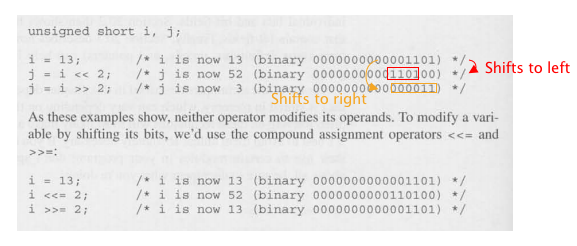
\includegraphics[width=0.9\linewidth]{images/review_9_solution_1.png}
            \end{center}

            \item \texttt{$>>=$} / \texttt{$<<=$} : Are bitwise shift equivalent of \texttt{$+=$}
        \end{itemize}


    \end{itemize}
\end{enumerate}

\end{document}